\documentclass{beamer}
\usetheme{default}
%\setbeamercolor{structure}{bg=black,fg=white}
%\setbeamercolor{normal text}{bg=black,fg=white}
\setbeamercolor{structure}{fg=black,bg=white}
\setbeamercolor{normal text}{fg=black,bg=white}
\useoutertheme{umbcfootline}
\beamertemplateballitem % Fancy bullets
\newcommand{\ud}{\mathrm{d}} 
\newcommand{\degree}{$^{\circ}$}
\newcommand{\tb}[1]{\textcolor{blue}{#1}} 
\newcommand{\E}{\text{E}}

\usepackage{hyperref}

\title[Survey]{CSGF Survey Summary}
\author{Carl Boettiger}
\institute{UC Davis}
\date{\today}

\usepackage{rotating}
\usepackage{times}



\begin{document}
\begin{frame}
\titlepage
\end{frame}

\frame{\frametitle{Stumped you!}


How would you describe how you use ``None''
\begin{itemize}
\item[(a)] Never
\item[(b)] beginner
\item[(c)] regular user
\end{itemize}
}	

\section{Introduction}


\frame{\frametitle{Background on this Survey}
\pause
\begin{itemize}
\item Me = biologist
\pause
\item My first year at CSGF = clueless
\pause
\item My answers to the survey = ``Never heard of it''
\end{itemize}
	}

\frame{\frametitle{Themes}
\begin{enumerate}
\item How do we compute?  High level/low level?  Parallelization?  
\item Good Practices
\item Communication / Web 2.0
\item Breaking down by year, field, etc
\end{enumerate}
}

\section{Languages}
\frame{\frametitle{So what languages do we use?}

}

\frame{\frametitle{Compiled languages}
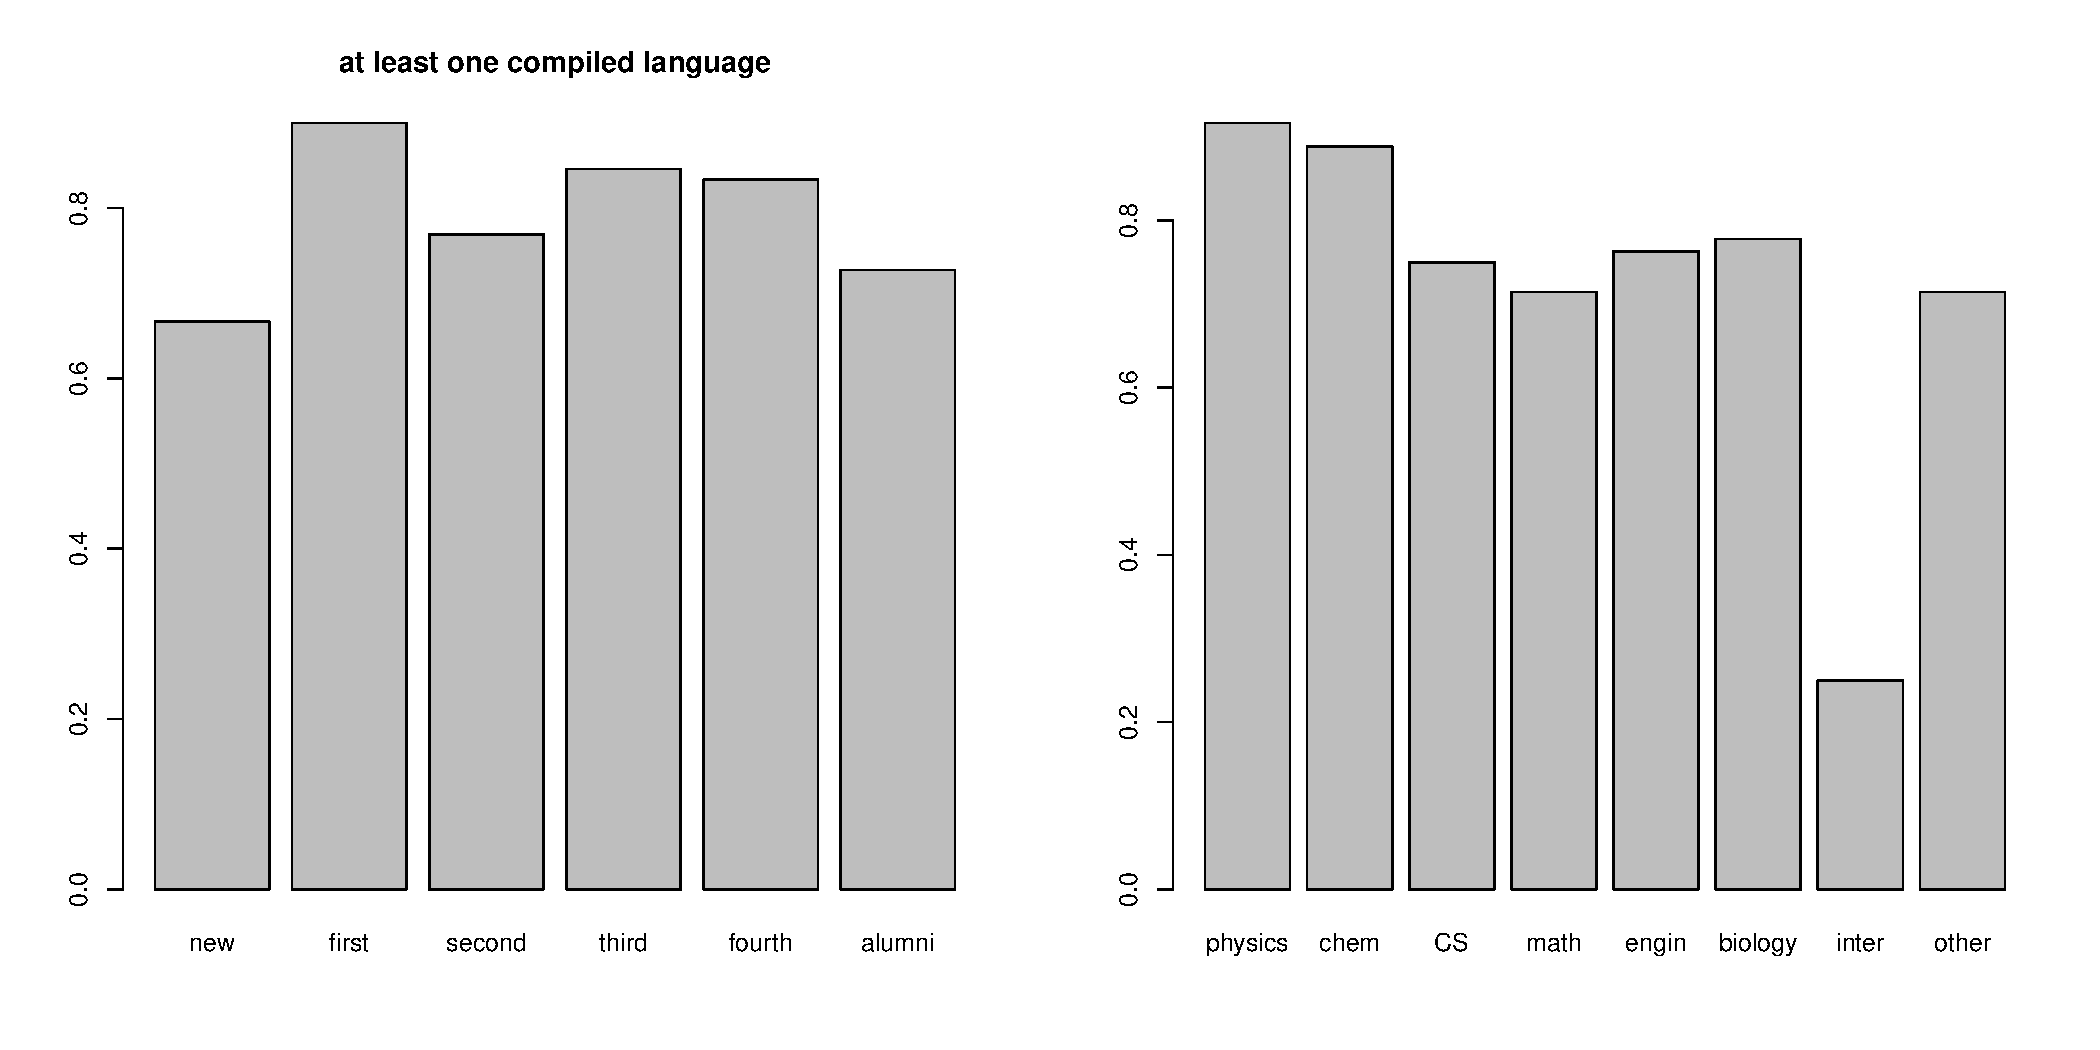
\includegraphics[width=\linewidth]{compiled.pdf}
}


\frame{\frametitle{Who uses Fortran77 ``regularly''?}
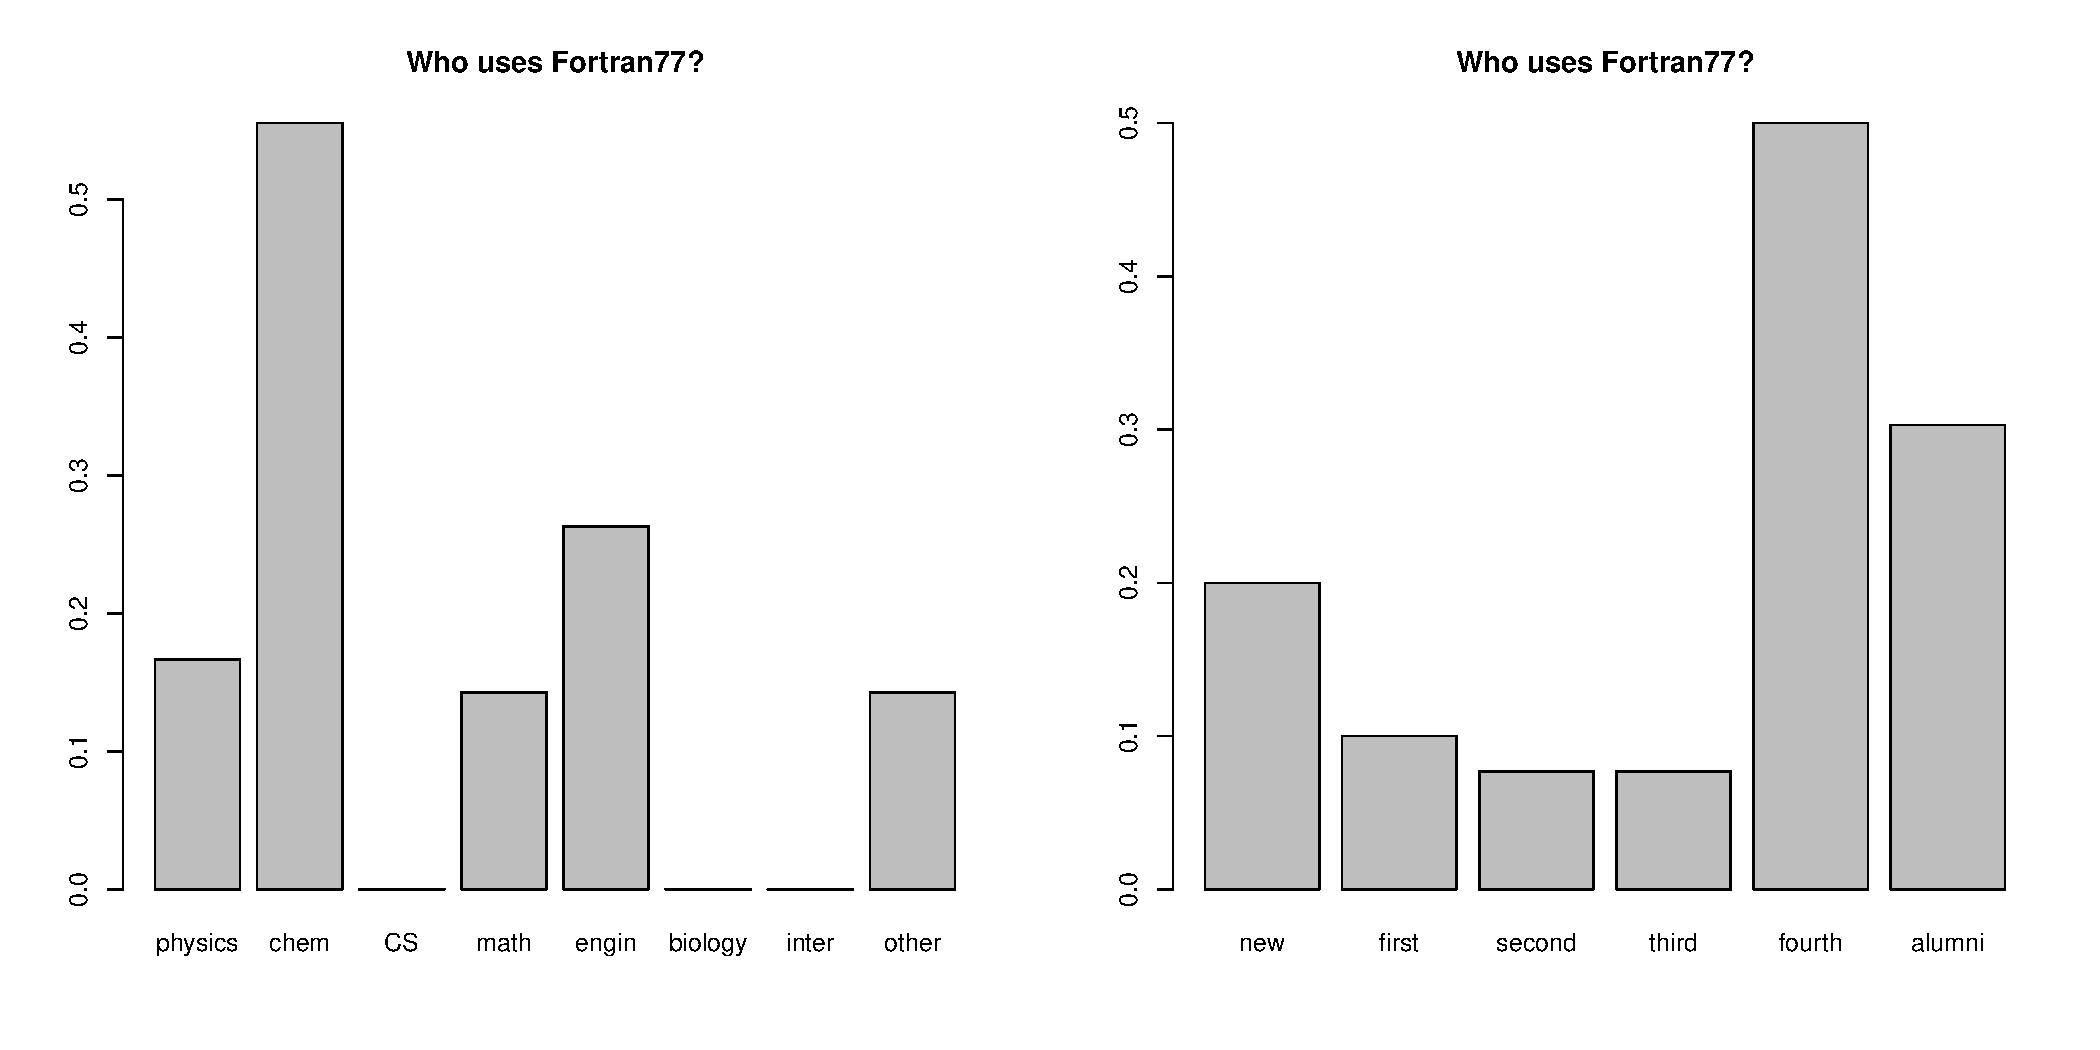
\includegraphics[width=\linewidth]{fortran77.pdf}
}

\frame{\frametitle{Mathematicians don't use Python}
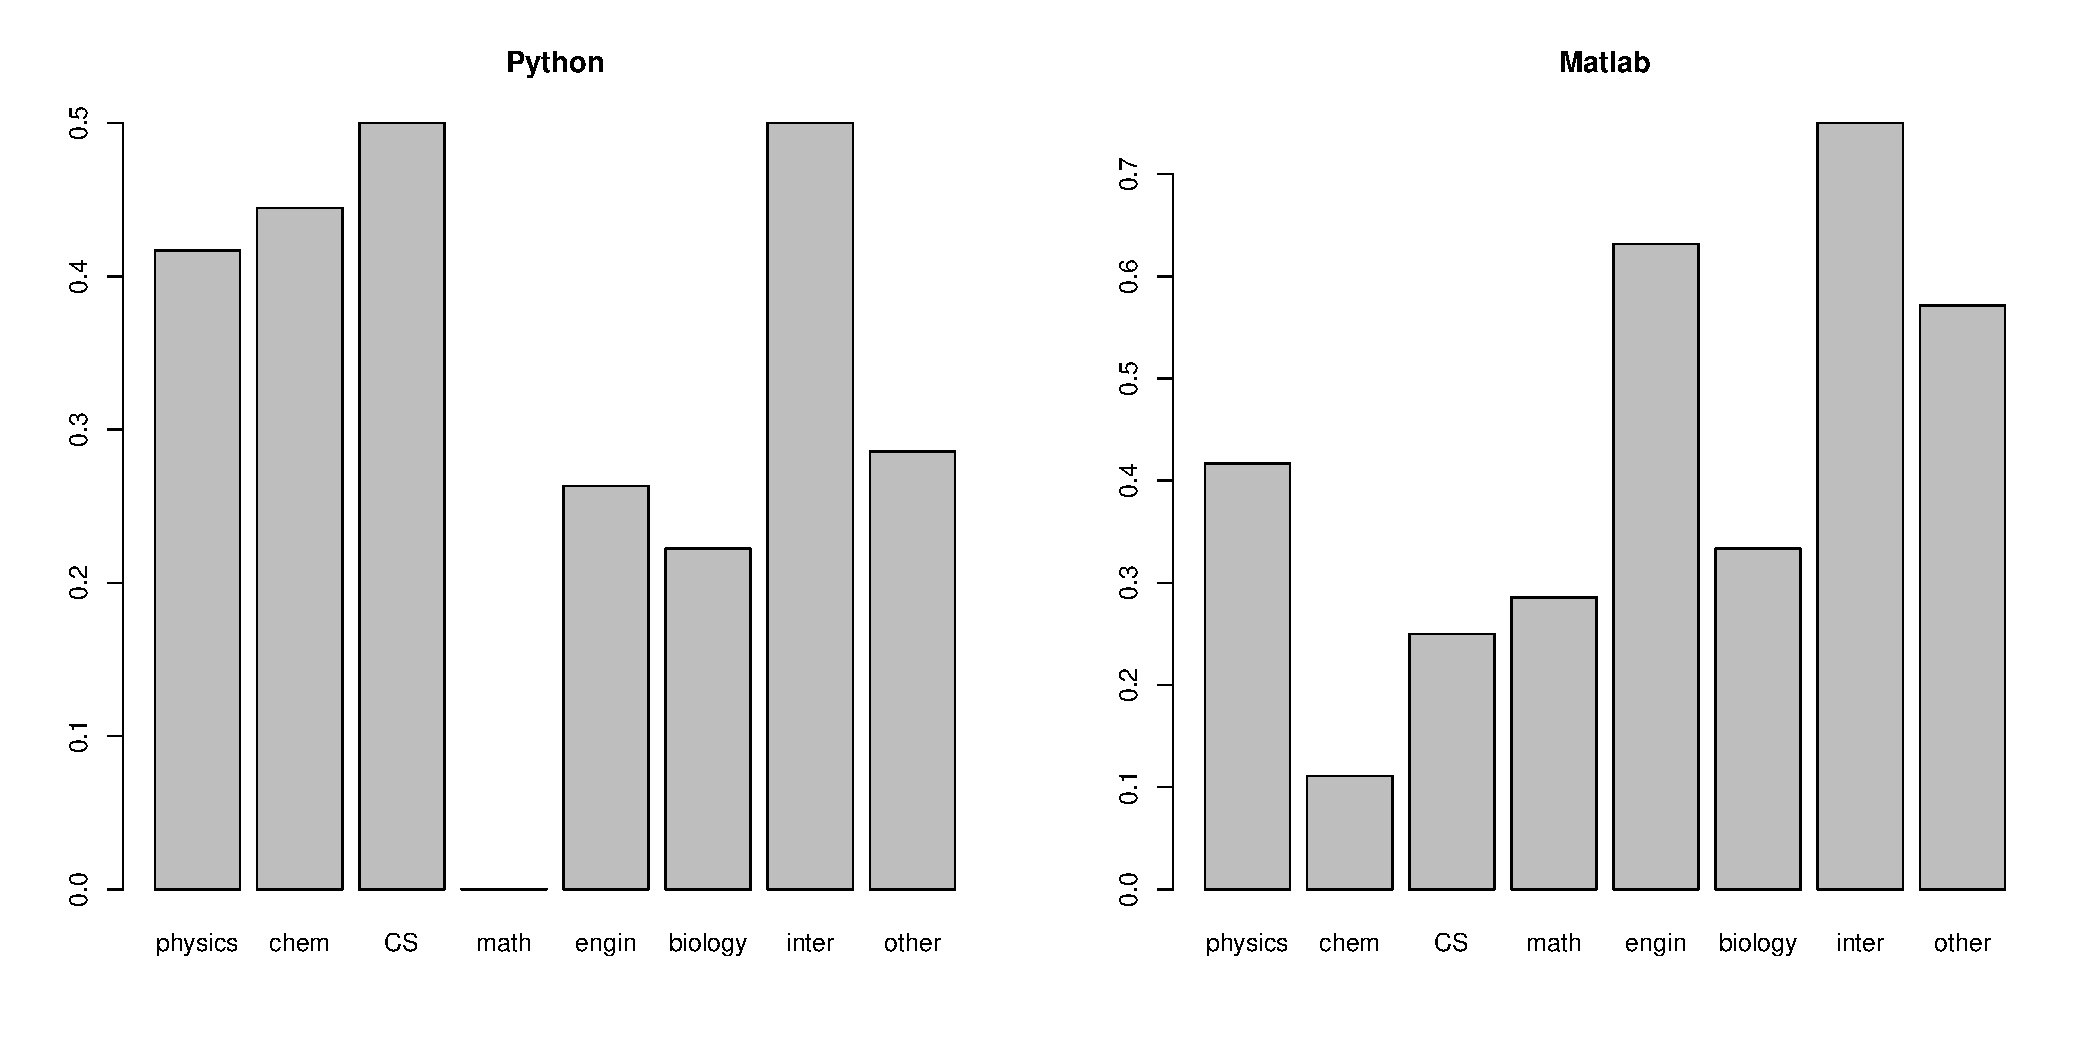
\includegraphics[width=\linewidth]{scripting}
}

\frame{\frametitle{Mathematicians don't use Python}
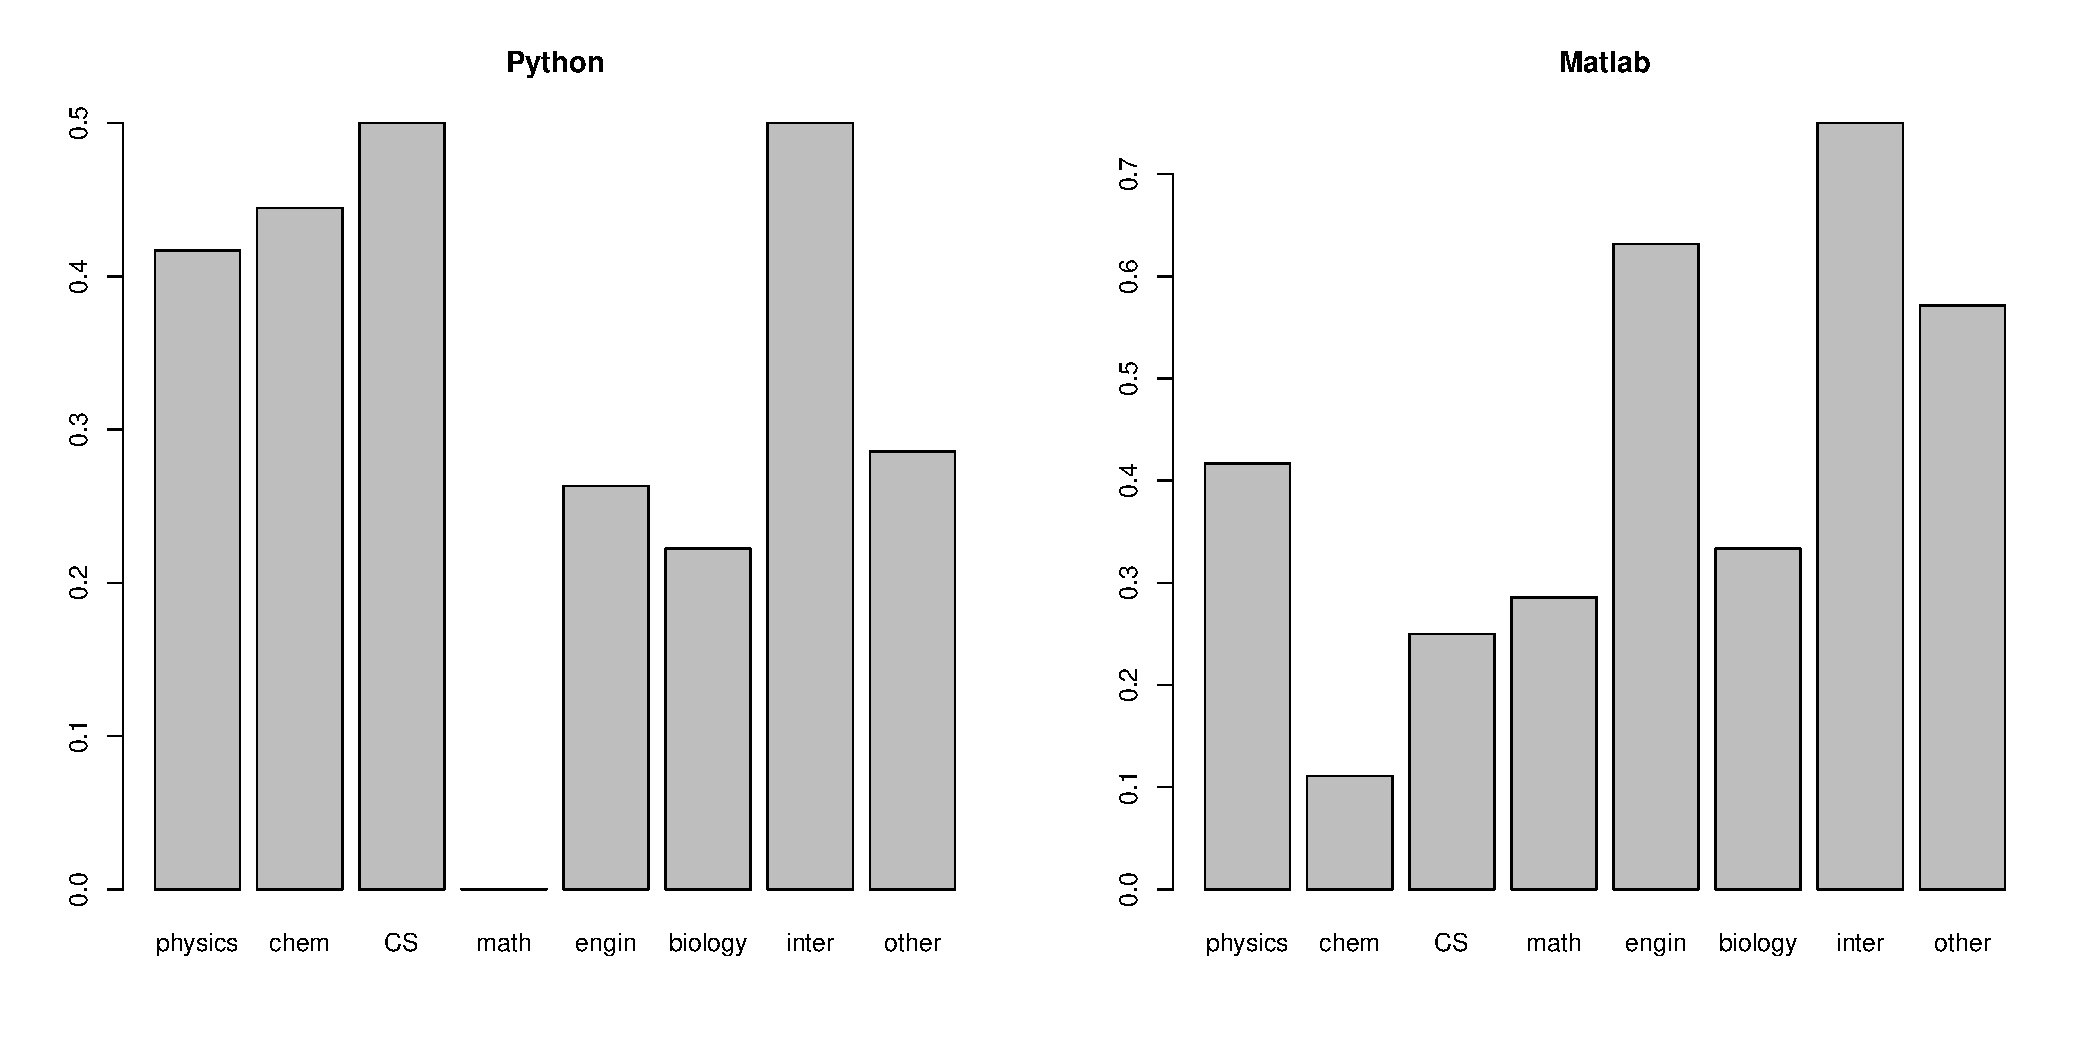
\includegraphics[width=\linewidth]{scripting}
}

\frame{\frametitle{\ldots then you're probably a physicist}
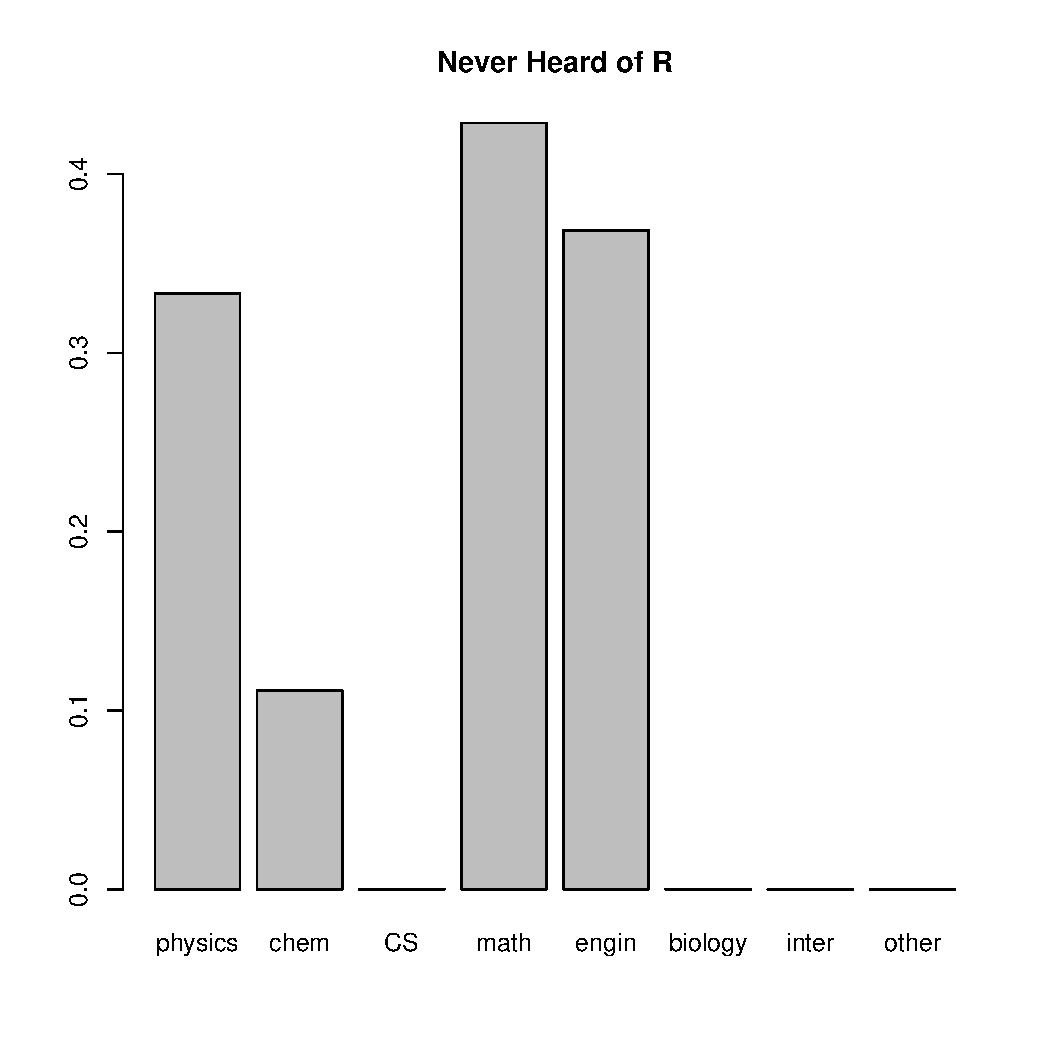
\includegraphics[width=.75\linewidth]{R}
}

\frame{\frametitle{which means you're either multilingual or schizophrenic}
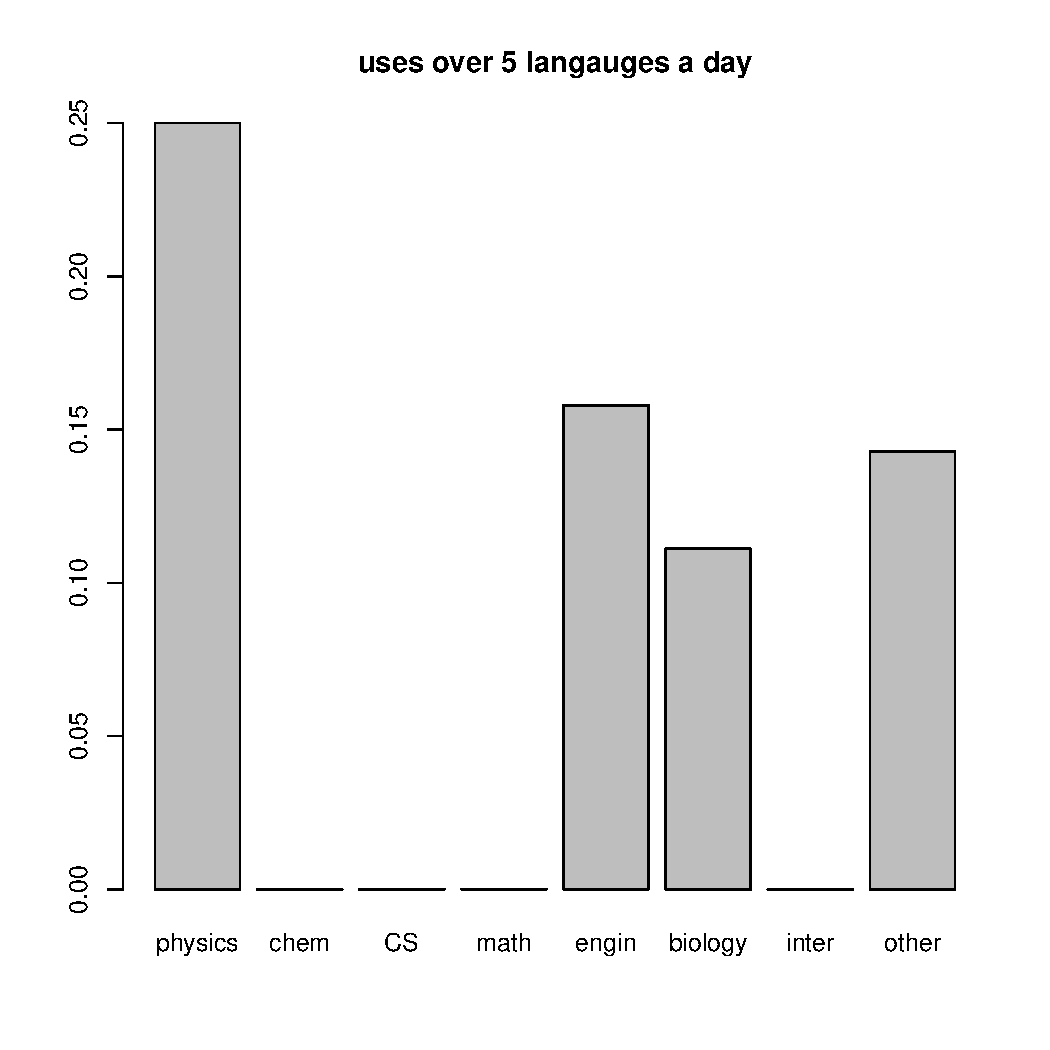
\includegraphics[width=.75\linewidth]{multilingual}
}

\frame{
	\Large{ How about Parallel code?}
}
\frame{\frametitle{Almost everyone uses at least occasionally!}
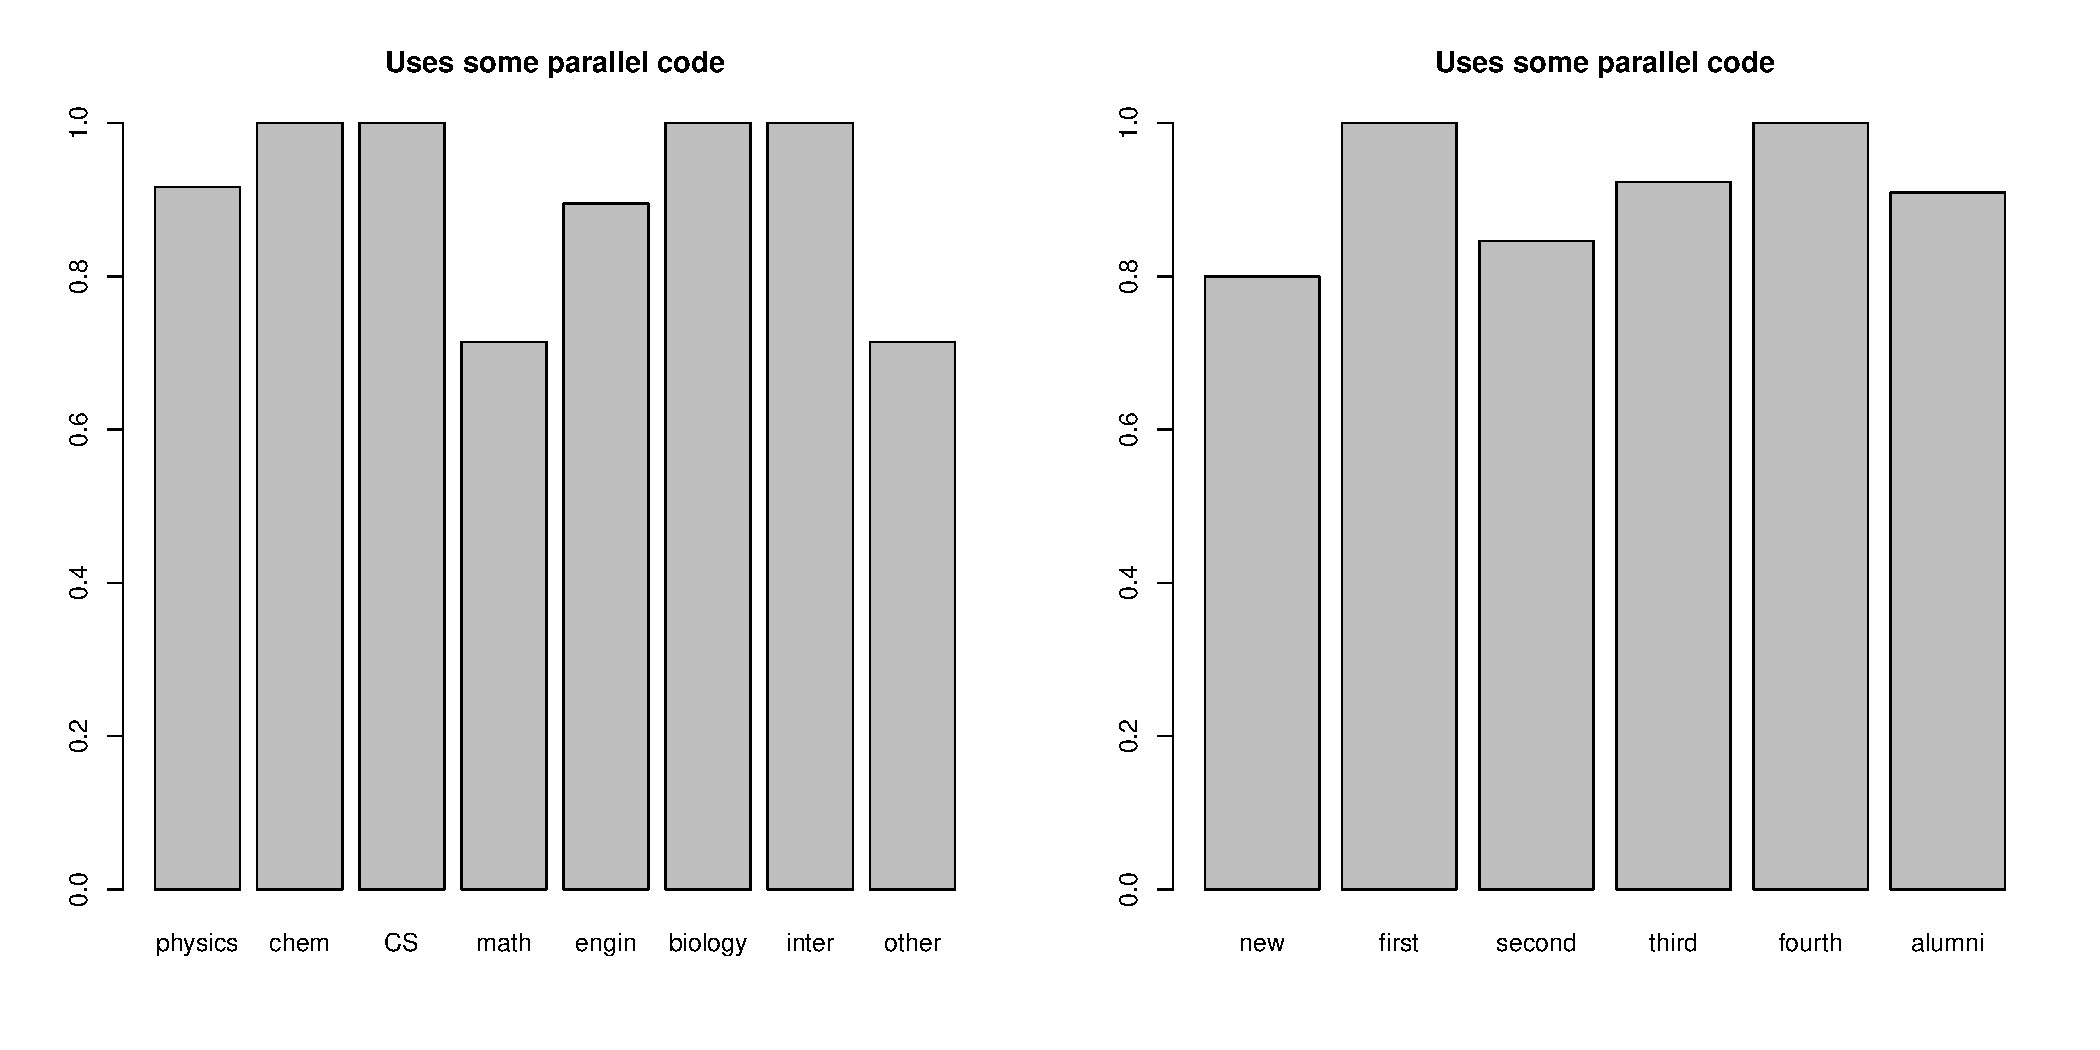
\includegraphics[width=\linewidth]{some_parallel}
}

\frame{\frametitle{And some get carried away}
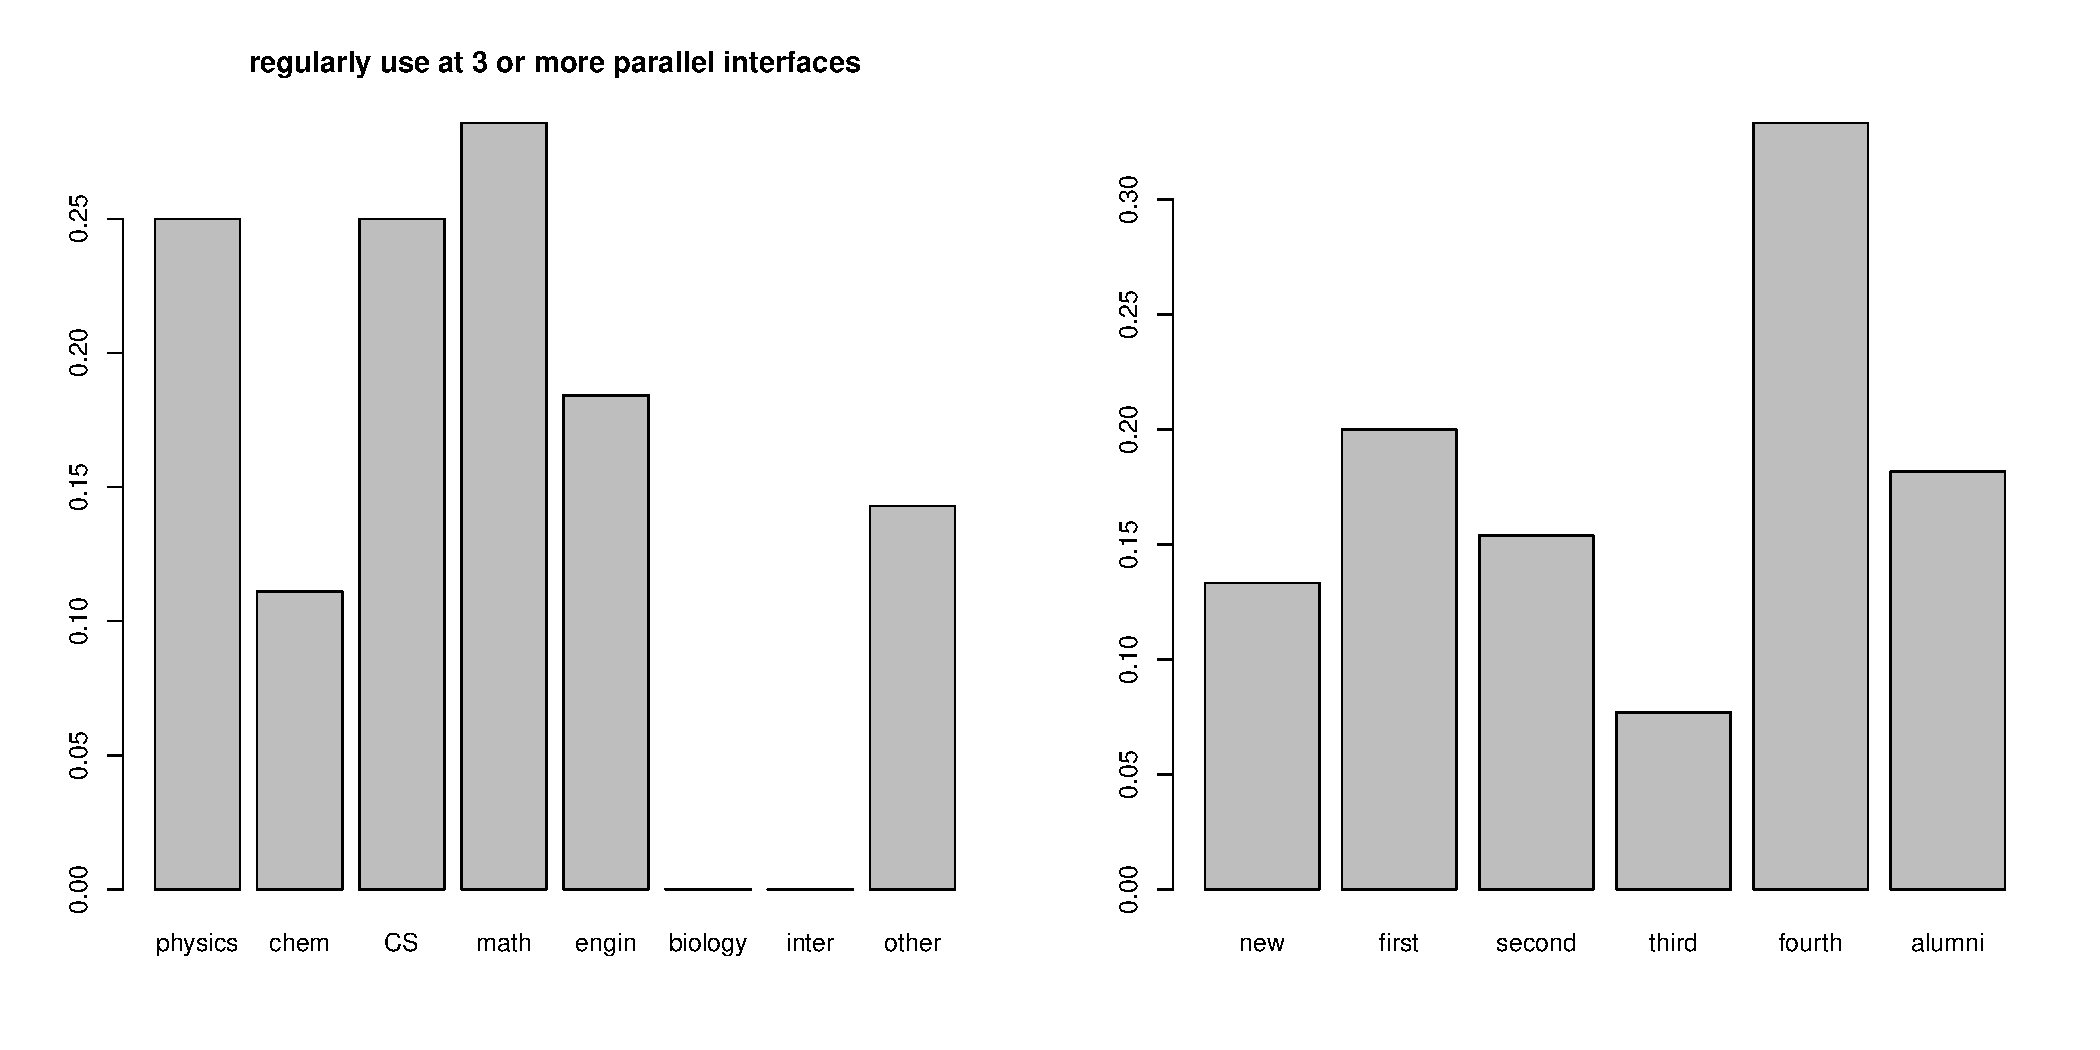
\includegraphics[width=\linewidth]{obsessed}
}

\frame{\frametitle{Over 25\% of us are exploring GPU computing}
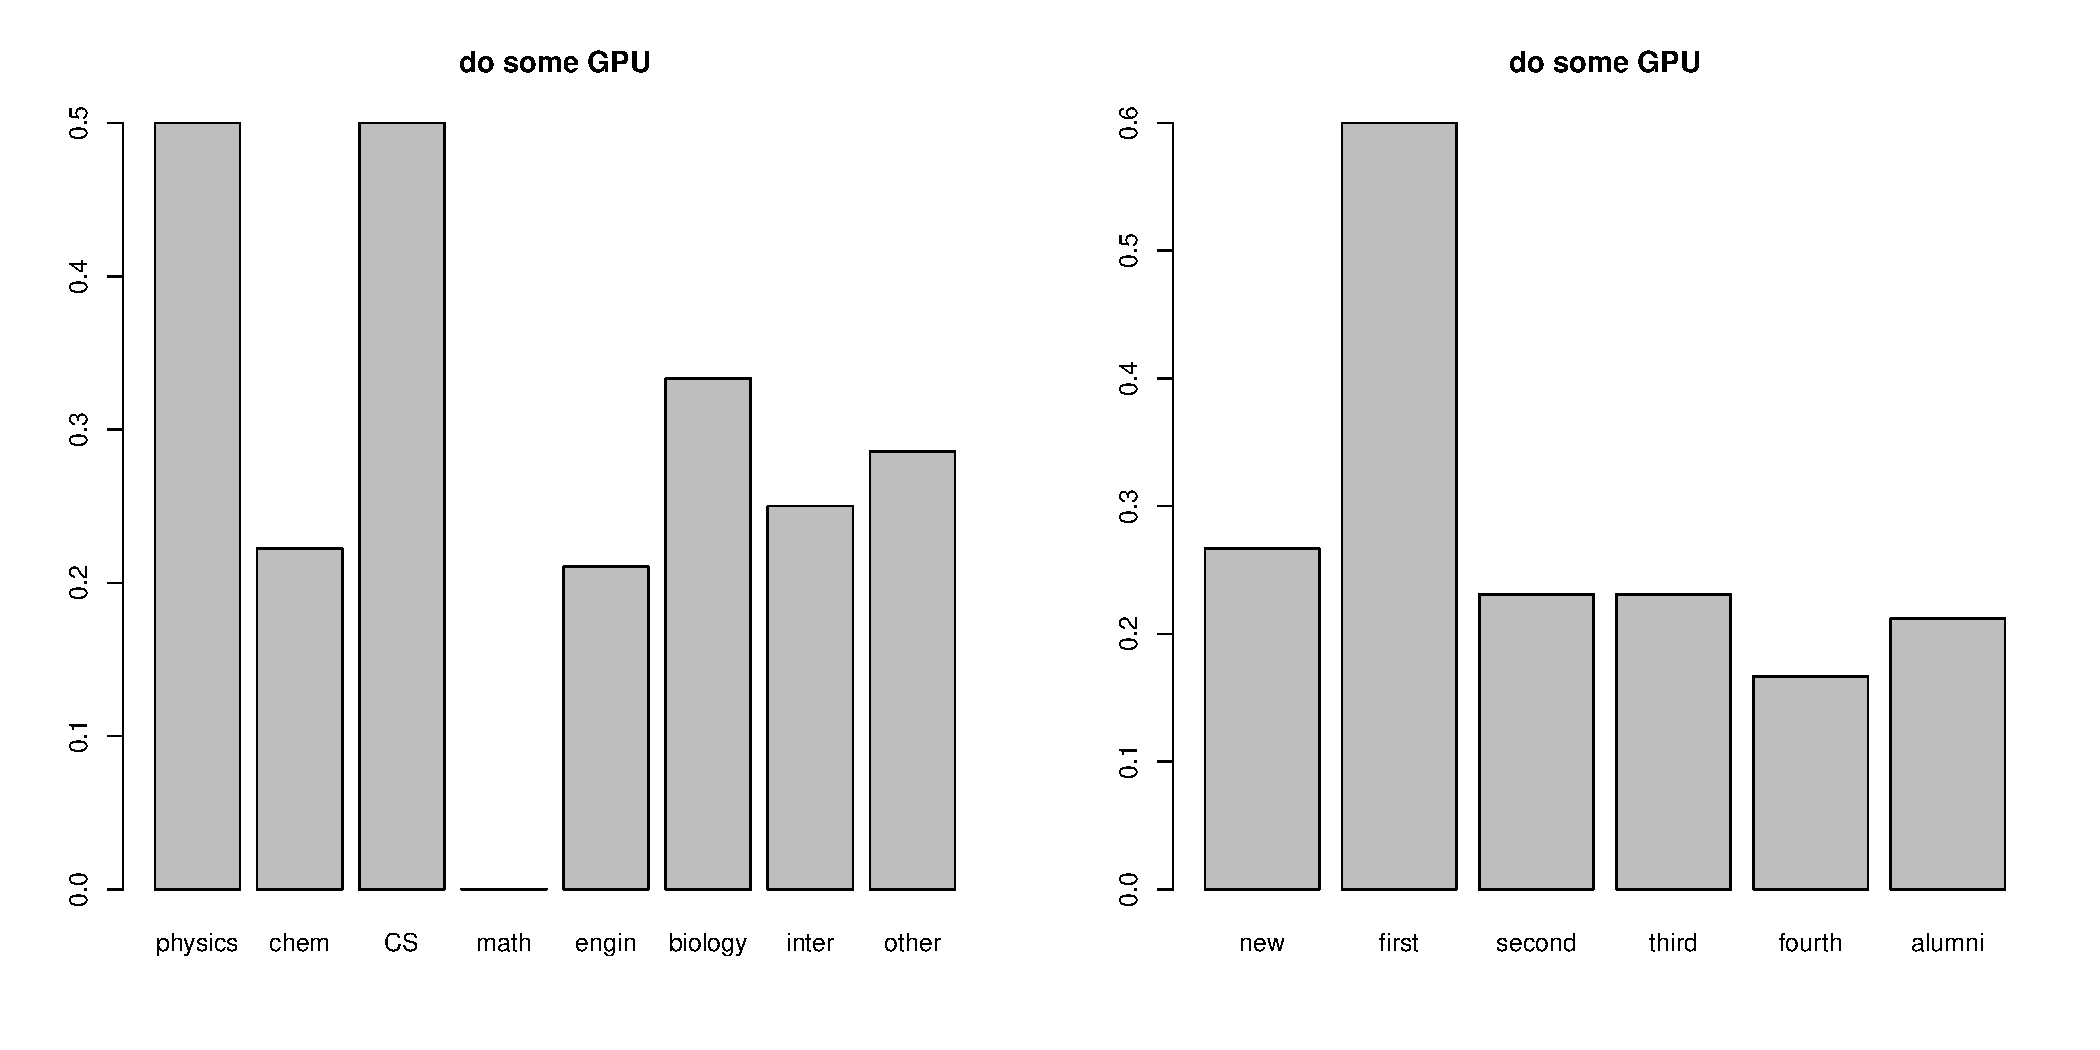
\includegraphics[width=\linewidth]{gpu}
}

\frame{
	We all use \LaTeX, we can get by in HTML, but don't ask us about web development!
}
\frame{ \frametitle{and our favorite operating system is\dots}
\pause
\begin{center}

\includegraphics[width=4cm]{tux}
\end{center}
}
\frame{ \frametitle{and our favorite operating system is\dots}
\begin{center}
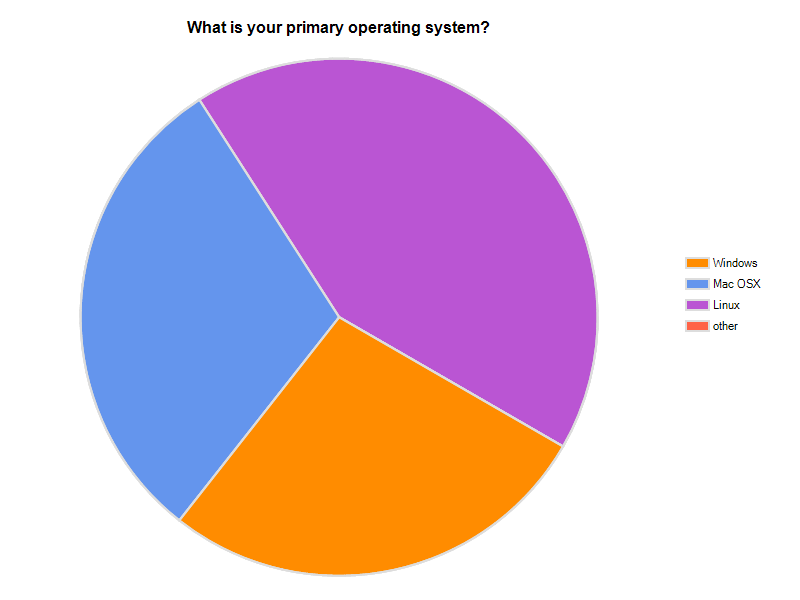
\includegraphics[width=.7\linewidth]{os}
\end{center}
}



\section{Good Practices}
\frame{
	\begin{center}
	\LARGE II.  Good Software Practices
	\end{center}
}

\frame{ \frametitle{Software Carpentry Quiz}
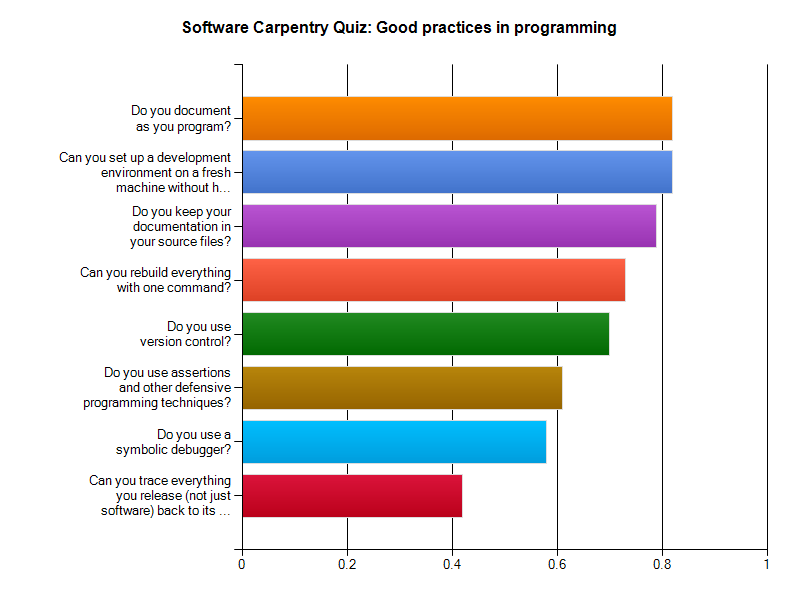
\includegraphics[width=\linewidth]{good_practices}
}
\frame{ \frametitle{Software Carpentry Quiz}
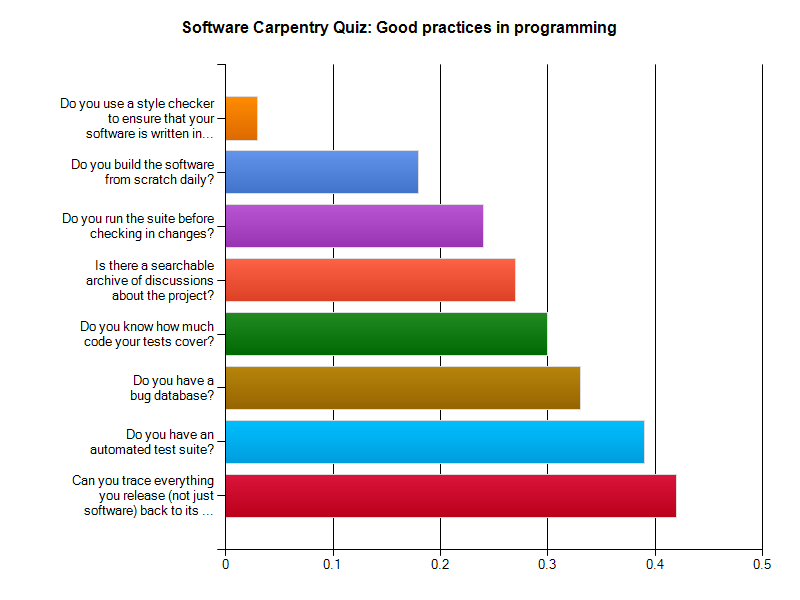
\includegraphics[width=\linewidth]{bad_practices}
}

\frame{\frametitle{No strong pattern here by year or PhD\dots}
How about having been on practicum?
\pause 
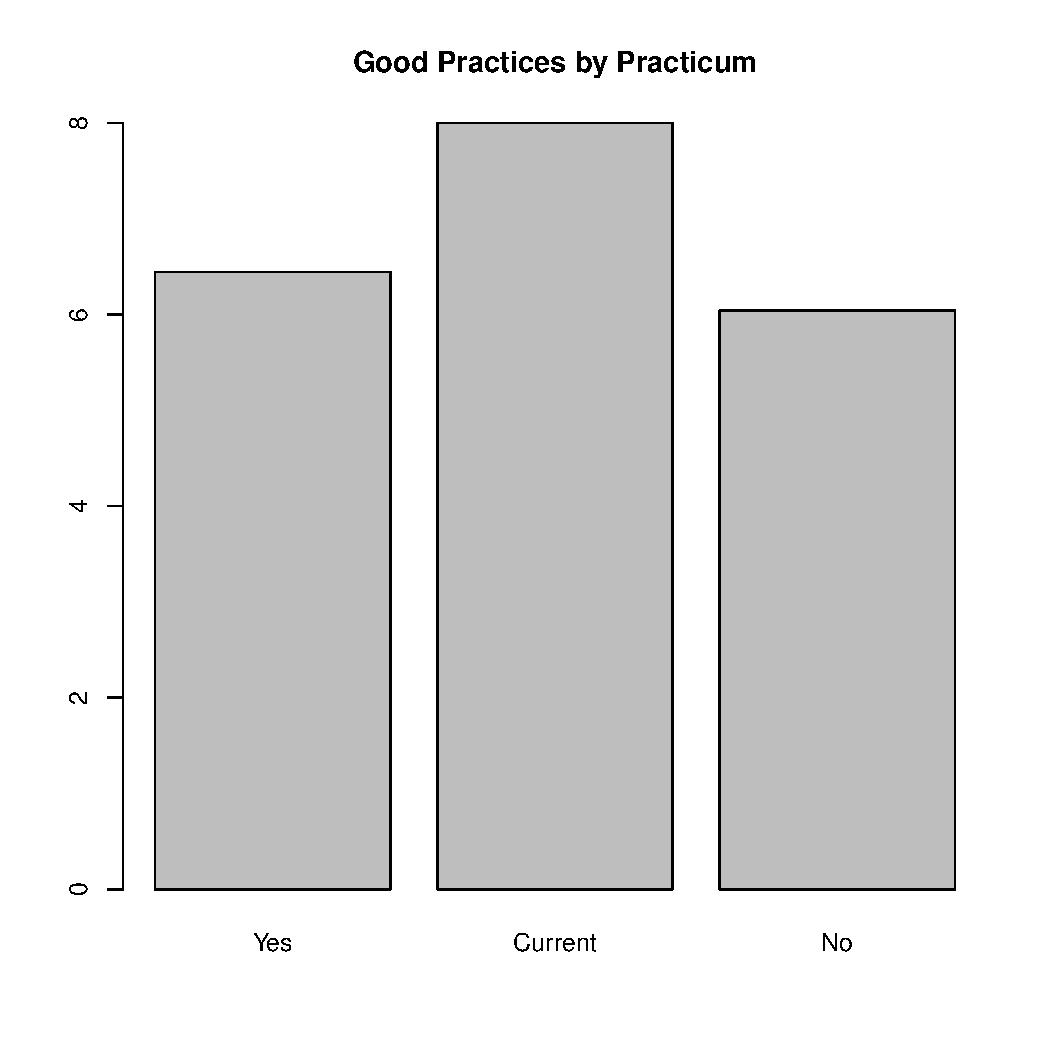
\includegraphics[width=.7\linewidth]{carpentry}
}

\frame{
\begin{itemize}
\item Version management: Mostly subversion, some cvs
\item Documentation: Mostly by detailed comments.  Some Doxygen, 1/4 use self documenting and readme's.  
\end{itemize}
}


\frame{\frametitle{Visualization}
We mostly visualize with stuff we've never heard of\dots
\vspace{-.3in}
\begin{center}
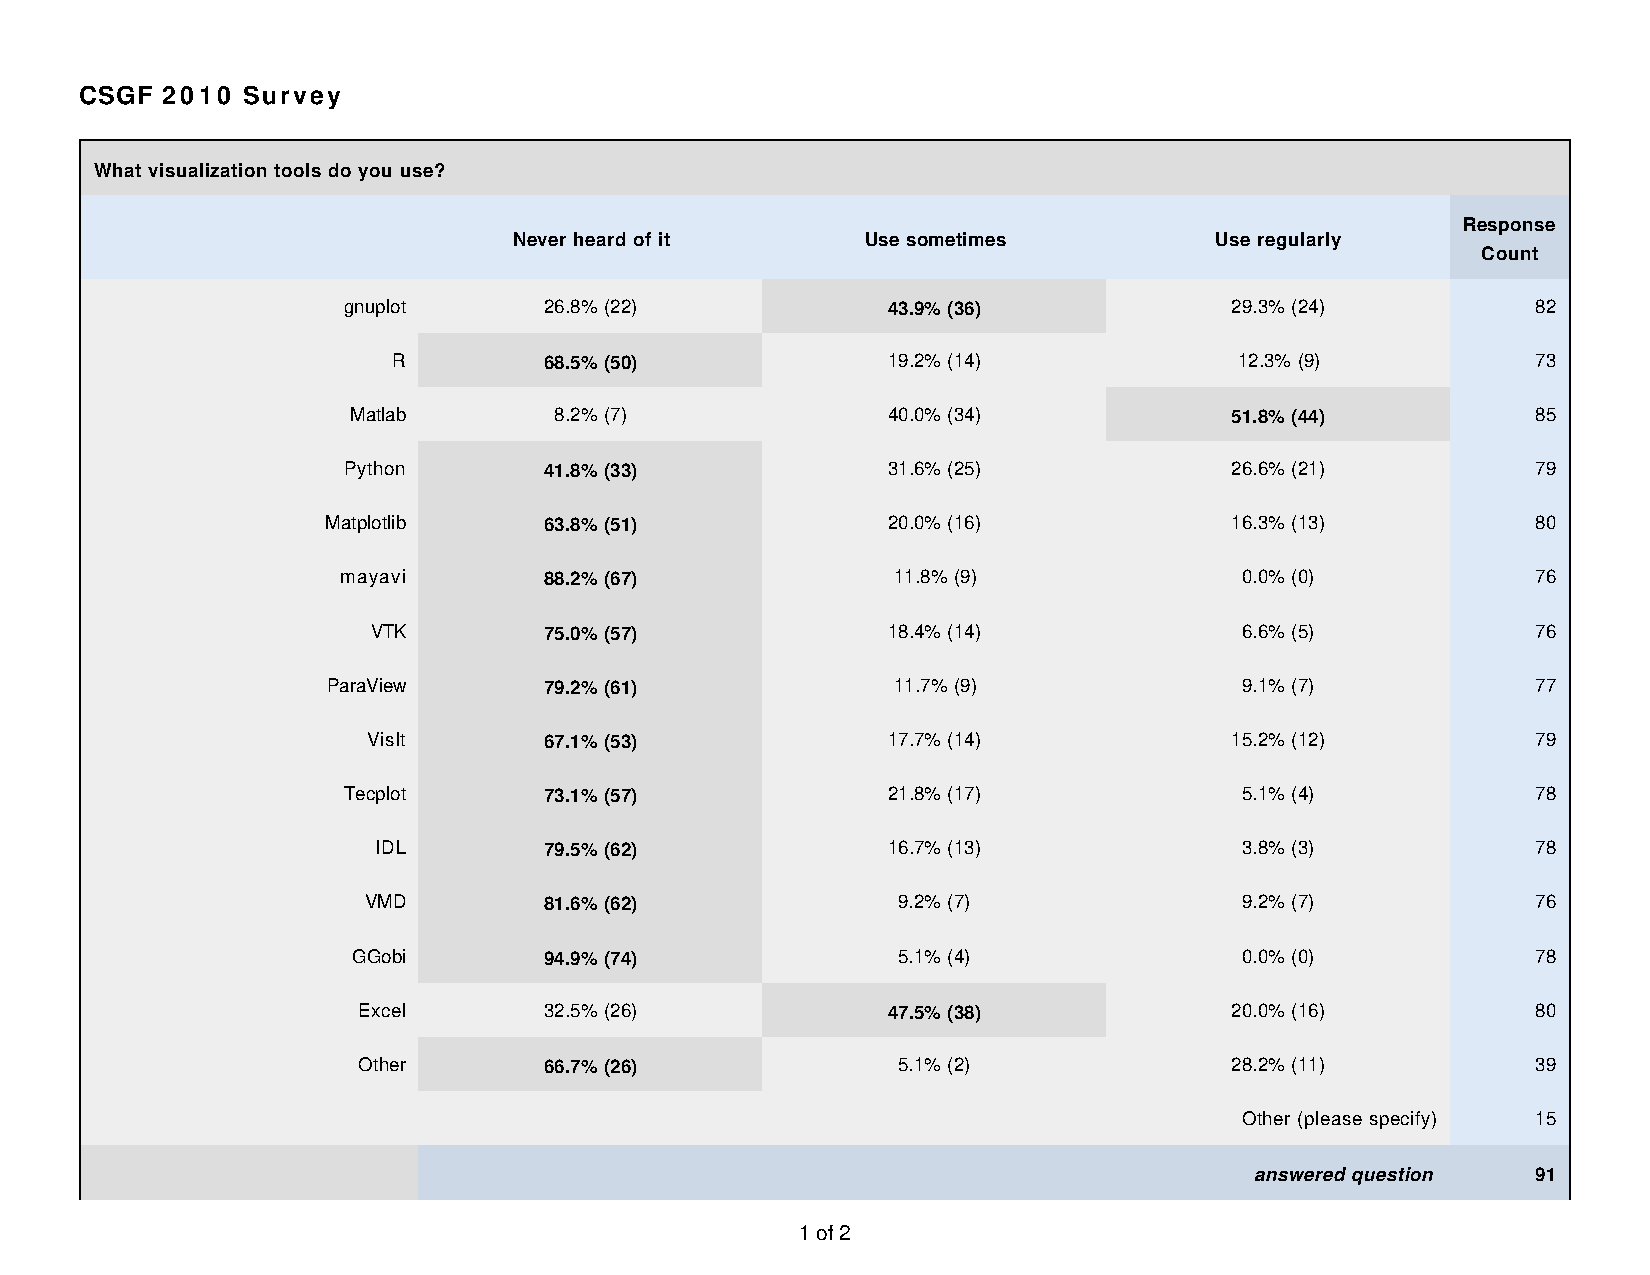
\includegraphics[width=\linewidth]{visualize}
\end{center}
}

\section{Communication \& Web 2.0}
\frame{
	\begin{center}
	\LARGE III.  Communication / Web 2.0 tools
	\end{center}
}

\frame{\frametitle{Collaborations}
We're quite collaborative \dots
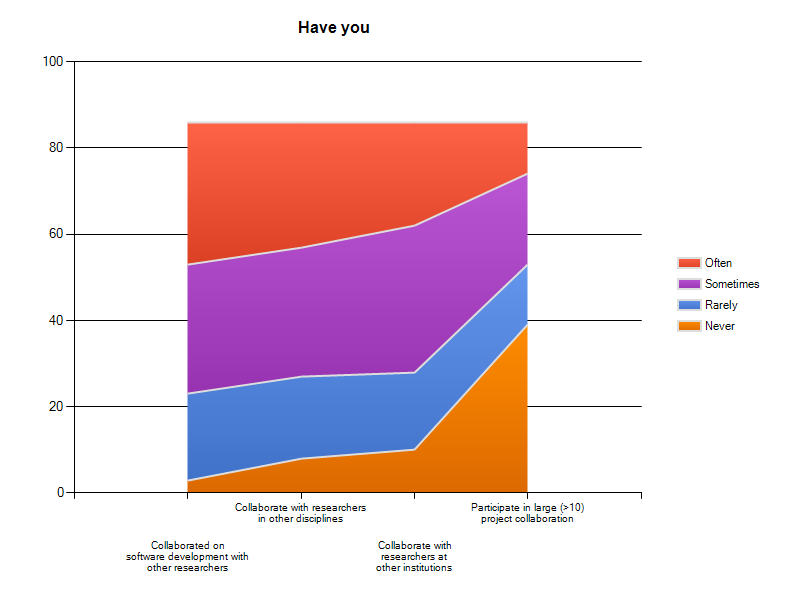
\includegraphics[width=\textwidth]{collab}
}

\frame{\frametitle{\dots but socially illiterate?}
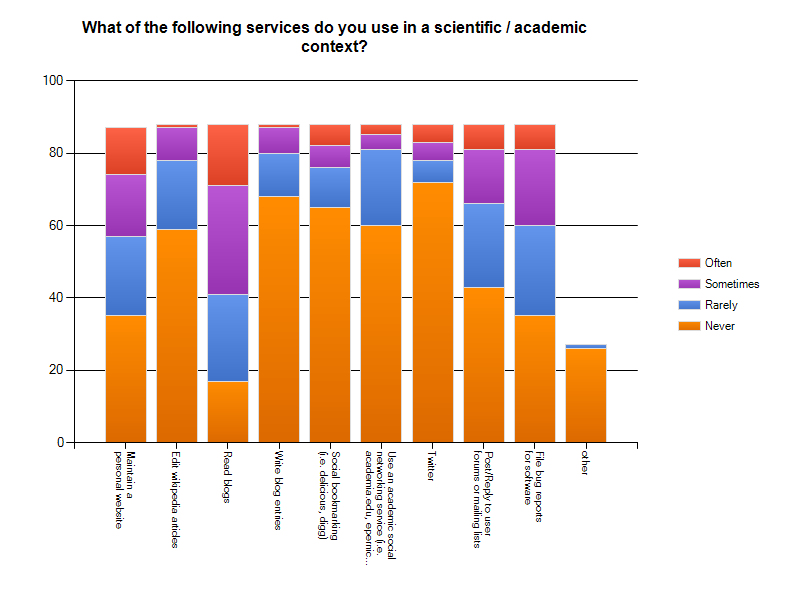
\includegraphics[width=\textwidth]{social}

\footnotesize{Few even have a website, but some follow blogs or file bug reports.}
}

\frame{\frametitle{Read what?}
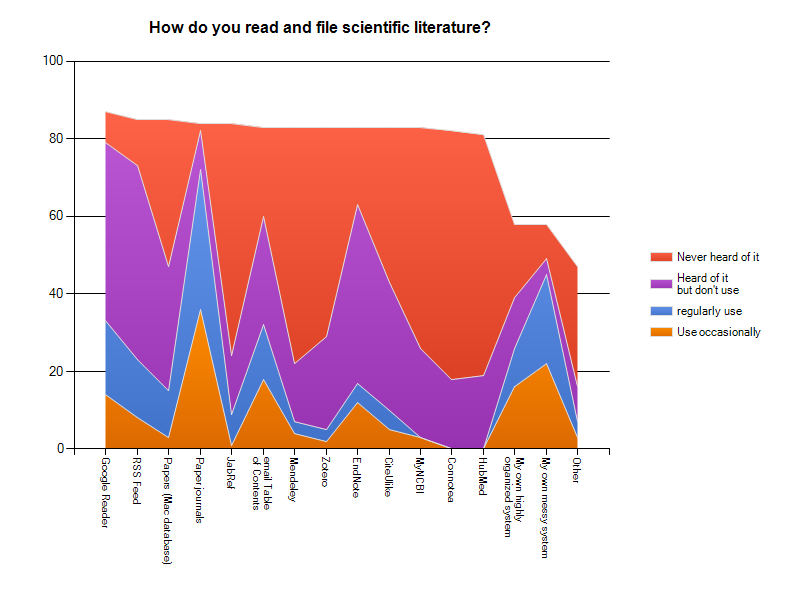
\includegraphics[width=\linewidth]{reading}
}

\frame{\frametitle{Somewhat open}
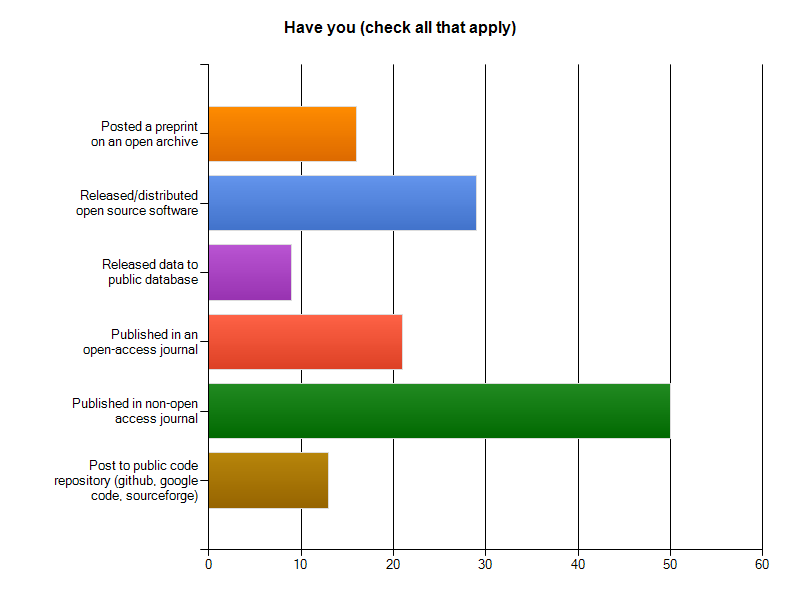
\includegraphics[width=\textwidth]{open}

}



\frame{\frametitle{Explore further!}
The data, along with a few functions in R that I've used to produce the plots can be downloaded from:
\vspace{1cm}
\begin{center}
\url{http://github.com/cboettig/sandbox/tree/master/csgf_survey/}
\end{center}
}

\end{document}

